\subsection{ROB}\label{sec:rob}

The ROB keeps all the in-flight instructions that have been renamed but not committed.
Instructions are enqueued into ROB in order at the renaming stage, and are dequeued from the ROB in order at the commit stage.
Instructions in the execution pipeline will also access the corresponding ROB entry.

\subsubsection{Interface}

\begin{figure}[!htb]
\begin{lstlisting}[caption={}]
typedef struct {
  Addr               pc;
  IType              iType;
  Maybe#(CSR)        csr;
  Bool               claimed_phy_reg;
  Maybe#(Trap)       trap;
  PPCVAddrCSRData    ppc_vaddr_csrData;
  Bit#(5)            fflags;
  Bool               will_dirty_fpu_state;
  RobInstState       rob_inst_state;
  LdStQTag           lsqTag;
  Maybe#(LdKilledBy) ldKilled;
  Bool               memAccessAtCommit;
  Bool               lsqAtCommitNotified;
  Bool               nonMMIOStDone;
  Bool               epochIncremented;
  SpecBits           spec_bits;
} ToReorderBuffer deriving(Bits, Eq, FShow);
\end{lstlisting}
\caption{Fields in an ROB entry}\label{fig:rob-entry}
\end{figure}

Before introducing the interface of the module, we first explain the fields in an ROB entry.
Figure~\ref{fig:rob-entry} shows the definition of type \code{ToReorderbuffer} which is a struct that contains all the fields in an ROB entry.
Now we explain each field (``the instruction'' refers to the instruction in the ROB entry):
\begin{itemize}
    \item \code{pc}: is the PC of the instruction.
    It is set when the renaming stage enqueues the instruction into ROB.
    
    \item \code{iType}: is the type (e.g., ALU, load, store, etc.) of the instruction.
    It is set when the renaming stage enqueues the instruction into ROB.
    
    \item \code{csr}: is the CSR index to access if the instruction is a \inst{CSRRW} instruction.
    It is set when the renaming stage enqueues the instruction into ROB.
    
    \item \code{claimed\_phy\_reg}: is true if the instruction has claimed a physical register to rename a architectural register.
    It is set when the renaming stage enqueues the instruction into ROB.
    If this field is true, then the instruction needs to release the originally mapped physical register for the renamed architectural register at commit stage.
    This field is always true unless the instructions represents an interrupt (we detect interrupts at renaming stage and encode an interrupt as an instruction in ROB) or the instruction has got an exception before being enqueued into ROB.
    
    \item \code{trap}: is the exception or interrupt associated with the instruction.
    It is set when the renaming stage enqueues the instruction into ROB, or when the memory instruction is dequeued from LSQ and it has triggered a memory page fault (or memory access fault) before.
    
    \item \code{ppc\_vaddr\_csrData}: is a tagged union.
    The field is initially set to the predicted next PC when the instruction is enqueued into ROB at the renaming stage.
    If the instruction is a memory instruction, then the field will be set to the virtual memory address after address translation.
    The virtual address will be used at the commit stage if the instruction triggers a page fault or access fault.
    If the instruction is a \inst{CSRRW} instruction that performs a read-modify-write on an CSR, then the field will be set to the original value of the CSR when the instruction leaves the ALU execution pipeline.
    If the instruction is a branch instruction, then the field will set to the computed next PC when the instruction leaves the ALU execution pipeline.
    
    \item \code{fflags}: is the status flags (e.g., overflow and underflow) of the FPU computation performed by the instruction in case the instruction is an FPU instruction.
    It is set when the FPU computation is done in the execution pipeline.
    It will be used at the commit stage to update an CSR for FPU.
    
    \item \code{will\_dirty\_fpu\_state}: is true if the destination register of the instruction is an floating point register.
    It is set when the instruction is enqueued into ROB at the renaming stage.
    It will be used at the commit stage to update an CSR for FPU.
    
    \item \code{rob\_inst\_state}: is a single bit to represent if the instruction has finished execution or not.
    Its value is either \code{Executed} or \code{NotDone}.
    
    \item \code{lsqTag}: is the index to LSQ if the instruction is a memory or fence instruction.
    
    \item \code{ldKilled}: is valid if the instruction is a load which is killed because the load speculation violates store-to-load memory dependency or memory ordering required by the consistency model.
    When the field is invalid, it also records the detailed reason for the kill of the load.
    It is set when the load instruction is dequeued from LSQ.
    
    \item \code{memAccessAtCommit}: is true if the memory or fence instruction must be executed non-speculatively, i.e., the instruction is a fence, an MMIO or an atomic (i.e., load-reserve, store-conditional and read-modify-write).
    It is set when the instruction finishes translating address.
    If this field is true, the instruction needs to notify LSQ when the instruction reaches the commit slot of the ROB (i.e., becomes the oldest in ROB).
    LSQ can issue this instruction to memory only after receiving the notification.
    
    \item \code{lsqAtCommitNotified}: is true if the instruction has already notified LSQ about reaching the commit slot of ROB.
    (This field is meaningful only if the \code{memAccessAtCommit} field is true.)
    It prevents repeated notifications to the LSQ.
    It is set when the notification to LSQ happens.
    
    \item \code{nonMMIOStDone}: is true if the instruction is a non-MMIO store and has translated its address and has computed its data, i.e., the store can be considered as executed even though it has not been issued to memory.
    If this field is true, then the instruction needs to notify LSQ when it is dequeued from ROB at the commit stage.
    (The \code{lsqAtCommitNotified} field does not need to be set because the entry is already dequeued from ROB.)
    This field is set when the instruction finishes translating address.
    
    \item \code{epochIncremented}: is true if the instruction has incremented the epoch at the renaming stage to drop any future instructions from the fetch stage.
    This field is true only when the instruction represents an interrupt, is a system instruction that needs to be performed in a blocking way, or triggers an exception before being enqueued into ROB.
    If this field is true, then when this instruction is committed, the commit stage does not need to increment the epoch at the renaming stage again when redirecting the fetch stage (the epoch at the fetch stage still needs to be incremented).
    This field is set when the renaming stage enqueues the instruction into ROB.
    
    \item \code{spec\_bits}: is the bit mask to encode all the older unresolved branches (Section~\ref{sec:specupdate}).
    This field is in fact not truly used in squashing wrong-path instructions, because ROB keeps all instructions in order and squash can be performed according to the ROB index of the mispredicted branch.
    It is kept for sanity checks in simulation.
\end{itemize}

\begin{figure}[!htb]
\begin{lstlisting}[caption={}]
// InstTag is the index to access an ROB entry
// ControlFlow is a struct that contains the computed next PC
interface ROB_EnqPort;
  method Bool canEnq;
  method Action enq(ToReorderBuffer x);
  method InstTag getEnqInstTag;
endinterface
interface ROB_DeqPort;
  method Bool canDeq;
  method Action deq;
  method InstTag getDeqInstTag;
  method ToReorderBuffer deq_data;
endinterface
interface ROB_setExecuted_doFinishAlu;
  method Action set(InstTag x, Maybe#(Data) csrData, ControlFlow cf);
endinterface
interface ROB_setExecuted_doFinishFpuMulDiv;
  method Action set(InstTag x, Bit#(5) new_fflags);
endinterface
interface ROB_getOrigPC;
  method Addr get(InstTag x);
endinterface
interface ROB_getOrigPredPC;
  method Addr get(InstTag x);
endinterface
interface ROB_SpeculationUpdate;
  method Action incorrectSpeculation(Bool kill_all, SpecTag spec_tag, InstTag inst_tag);
  method Action correctSpeculation(SpecBits mask);
endinterface
\end{lstlisting}
\caption{Subinterfaces of ROB}\label{fig:rob-subifc}
\end{figure}

\begin{figure}[!htb]
\begin{lstlisting}[caption={}]
// SupSize is the superscalar size
// InstTime is the conceptual ROB index if ROB were implemented using a circular buffer
interface SupReorderBuffer#(numeric type aluExeNum, numeric type fpuMulDivExeNum);
  interface Vector#(SupSize, ROB_EnqPort) enqPort;
  method Bool isEmpty;
  interface Vector#(SupSize, ROB_DeqPort) deqPort;
  method Action setLSQAtCommitNotified(InstTag x);
  method Action setExecuted_deqLSQ(InstTag x, Maybe#(Exception) cause, Maybe#(LdKilledBy) ld_killed);
  interface Vector#(aluExeNum, ROB_setExecuted_doFinishAlu) setExecuted_doFinishAlu;
  interface Vector#(fpuMulDivExeNum, ROB_setExecuted_doFinishFpuMulDiv) setExecuted_doFinishFpuMulDiv;
  method Action setExecuted_doFinishMem(InstTag x, Addr vaddr, Bool access_at_commit, Bool non_mmio_st_done);
  interface Vector#(aluExeNum, ROB_getOrigPC) getOrigPC;
  interface Vector#(aluExeNum, ROB_getOrigPredPC) getOrigPredPC;
  method InstTime getEnqTime;
  interface ROB_SpeculationUpdate specUpdate;
endinterface
module mkSupReorderBuffer(SupReorderBuffer#(aluExeNum, fpuMulDivExeNum);
  // module implementation
endmodule
\end{lstlisting}
\caption{Interface of ROB}\label{fig:rob-ifc}
\end{figure}

Figures~\ref{fig:rob-subifc} and \ref{fig:rob-ifc} show the interface of ROB.
The interface parameters \code{aluExeNum} and \code{fpuMulDivExeNum} are the numbers of ALU execution pipelines and FPU execution pipelines, respectively.
Now we explain each method in the ROB interface (Figure~\ref{fig:rob-ifc}):
\begin{itemize}
    \item Subinterface \code{enqPort}: provides a vector of methods to enter instructions into ROB at the renaming stage.
    ROB-entry fields \code{ldKilled}, \code{lsqAtCommitNotified}, and \code{nonMMIOStDone} are self-initialized to false or invalid.
    Field \code{memAccessAtCommit} is self-initialized to true if the instruction is a fence.
    All other fields are initialized by taking directly the values from the method argument.
    The enqueue methods have to be called consecutively, i.e., it is legal to call \code{enqPort[0]} and then \code{enqPort[1]}, but it is illegal to skip \code{enqPort[0]} and directly call \code{enqPort[1]}.
    
    \item Subinterface \code{isEmpty}: return true if the ROB is empty.
    
    \item Subinterface \code{deqPort}: provides a vector of methods to dequeue instructions from ROB at the commit stage.
    The guard of the dequeue method only checks if the dequeuing entry is valid or not, i.e., the commit stage should check whether the instruction can really commit (e.g., has finished execution or not).
    Similar to \code{enqPort}, the dequeue methods also need to be called consecutively, i.e., cannot skip \code{deqPort[0]} and call \code{deqPort[1]} directly.
    
    \item Method \code{setLSQAtCommitNotified}: sets the \code{lsqAtCommitNotified} field to true.
    
    \item Method \code{setExecuted\_deqLSQ}: is called when a memory instruction which is not a non-MMIO store gets dequeued from LSQ (a non-MMIO store is dequeued from LSQ after it is dequeued from ROB).
    The method sets field \code{rob\_inst\_state} to \code{Executed}.
    It also sets field \code{trap} if \code{trap} is originally invalid and method argument \code{cause} is valid.
    It also sets field \code{ldKilled} if argument \code{ld\_killed} is valid.
    
    \item Subinterface \code{setExecuted\_doFinishAlu}: provides a vector of methods for instructions at the end of ALU execution pipelines to notify the ROB that execution is done.
    The method sets field \code{rob\_inst\_state} to \code{Executed}.
    If method argument \code{csrData} is valid (i.e., the instruction is \inst{CSRRW}), then it sets field \code{ppc\_vaddr\_csrData} to \code{csrData} (i.e., the original CSR value).
    Otherwise, it sets the field to the computed next PC contained in argument \code{cf}.
    
    \item Subinterface \code{setExecuted\_doFinishFpuMulDiv}: provides a vector of methods for instructions at the end of FPU execution pipelines to notify the ROB that execution is done.
    The method sets field \code{rob\_inst\_state} to \code{Executed}, and sets field \code{fflags} to method argument \code{new\_fflags}.
    
    \item Method \code{setExecuted\_doFinishMem}: is called by memory instructions that has translated their addresses.
    The method sets field \code{ppc\_vaddr\_csrData} to method argument \code{vaddr} (the virtual address of the memory address), sets field \code{memAccessAtCommit} to argument \code{access\_at\_commit}, and sets field \code{nonMMIOStDone} to argument \code{non\_mmio\_st\_done}.
    If argument \code{non\_mmio\_st\_done} is true, then it also sets field \code{rob\_inst\_state} to \code{Executed}.
    
    \item Subinterface \code{getOrigPC}: provides a vector of methods for instructions in the ALU pipeline to retrieve their PCs.
    
    \item Subinterface \code{getOrigPredPC}: provides a vector of methods for instructions in the ALU pipeline to retrieve the predicted next PCs (by the fetch stage) of them.
    
    \item Method \code{getEnqTime}: returns the conceptual enqueue pointer of ROB if ROB were implemented using a circular buffer.
    (ROB is implemented as a more complicated structure than a circular buffer, but it still behaves as if it were a circular buffer.)
    This method is called every cycle and the return value is passed to each reservation station to identify older instructions and prioritize them in issuing.
    
    \item Subinterface \code{specUpdate}: See Section~\ref{sec:specupdate}).
\end{itemize}

\noindent\textbf{Conflict Matrix:}
The conflict matrix of the interface methods are:
\begin{itemize}
    \item \code{deqPort[0]} $<$ $\cdots$ $<$ \code{deqPort[SupSize-1]} $<$ \code{setExecuted\_doFinishAlu[0]} $<$ $\cdots$ $<$ \code{setExecuted\_doFinishAlu[aluExeNum-1]} $<$ \code{setExecuted\_doFinishFpuMulDiv[0]} $<$ $\cdots$ $<$ \code{setExecuted\_doFinishFpuMulDiv[fpuMulDivNum-1]} $<$ \code{setExecuted\_deqLSQ} $<$ \code{setExecuted\_doFinishMem} $<$ \code{enqPort[0]} $<$ $\cdots$ $<$ \code{enqPort[SupSize-1]}
    \item \code{deqPort} $<$ \code{setLSQAtCommitNotified} $<$ \code{enqPort}
    \item \code{deqPort} $<$ \code{incorrectSpeculation} $<$ \code{correctSepculation}
    \item \code{incorrectSpeculation} C \code{enqPort}
    \item \code{enqPort} $<$ \code{correctSpeculation}
    \item All other pairs of methods are conflict free.
\end{itemize}

We order \code{deqPort} before everything else because \code{deqPort} is called at the commit stage which is the last stage in the processor pipeline.

We order \code{enqPort} after almost every other method because \code{enqPort} is called at the renaming stage while other methods are called at later stages.
The only exceptions are the \code{incorrectSpeculation} and \code{correctSpeculation} methods in the \code{specUpdate} subinterface.
We order \code{enqPort} before \code{correctSpecUpdate} because of the scheduling convention to put \code{correctSpecUpdate} at the last.
We make \code{enqPort} and \code{incorrectSpeculation} conflict because the newly enqueued instructions must be at the wrong path if ROB needs to be squashed.
We do not make \code{incorrectSpeculation} conflict with \code{deqPort} because they may be called together in the commit stage.
The ordering between \code{incorrectSpeculation} and \code{correctSpeculation} does not matter because they are never called in the same cycle.

The orderings between \code{setExecuted\_XXX} methods (we use \code{setExecuted\_XXX} to denote all the methods starting with \code{setExecuted}) are kind of arbitrary because these methods should be called for different instructions.
Nevertheless, we have to give an ordering for them because the BSC compiler believes they can write the same entry.
These orderings should be consistent with the orderings of the top-level rules that call these methods, and with the ordering of other modules called by these rules.
For example, we order \code{setExecuted\_deqLSQ} before \code{setExecuted\_doFinishMem} to match the conflict matrix of LSQ.

Although subinterface \code{getOrigPredPC} reads ROB-entry field \code{ppc\_vaddr\_csrData} which is written by \code{enqPort}, \code{setExecuted\_doFinishAlu} and \code{setExecuted\_doFinishMem}, we still make \code{getOrigPredPC} conflict free with all these methods.
This is because if these methods are called in the same cycle, they are guaranteed to access different ROB entries at the top level.
It should be noted that giving an ordering between \code{getOrigPredPC} and \code{setExecuted\_doFinishAlu} may create inefficiency.
Consider the case that we order \code{getOrigPredPC} after \code{setExecuted\_doFinishAlu} because \code{getOrigPredPC} is called in earlier pipeline stage.
Then, there is a bypass path from \code{setExecuted\_doFinishAlu} to \code{getOrigPredPC} which can never be activated.
Setting two methods as conflict free avoids this inefficiency.

A similar reasoning could explain why \code{getOrigPC} is conflict free with \code{enqPort}.
Since \code{getEnqTime} is just for determining the issue priority and does not affect correctness, we also make it conflict free with \code{enqPort}.

It should be noted that making \code{getOrigPredPC}, \code{getOrigPC} and \code{getEnqTime} before \code{enqPort} actually matches our scheduling convention (i.e., reverse pipeline order).
Thus, we may consider adding these orderings in future implementations.

\subsubsection{Implementation}
We use a set of EHRs to keep the content of an ROB entry, one EHR per field and an additional EHR for the valid bit.
Although the ROB entries are conceptually organized as a circular buffer, we do not implement it in that way.
The reason is to save the area for implementing superscalar enqueue and dequeue.
Consider the case that we implement ROB as a circular buffer, i.e., a vector of $N$ entries.
In this case, each dequeue/enqueue on the ROB will read/write one of the $N$ entries, costing $N$ units of area.
The total cost of implementing superscalar dequeue/enqueue is $N \times$\code{SupSize} units of area.
The way we implement the ROB can reduce this cost down to $N +O($\code{SupSize}$)$ units of area.

Figure~\ref{fig:rob-rotate-fifos} shows our implementation of ROB.
The ROB entries are organized as a \code{SupSize} FIFOs.
The enqueue port enqueues the FIFOs in a round-robin manner.
For example, consider the case \code{SupSize}=4, and initially ROB is empty.
At cycle 0, we perform 3 enqueues on FIFOs Q[0], Q[1], Q[2], respectively.
At cycle 1, if we perform 2 enqueues, then we will first enqueue Q[3] and then enqueue Q[0].
Dequeues are also performed in the round-robin manner.

\begin{figure}[!htb]
    \centering
    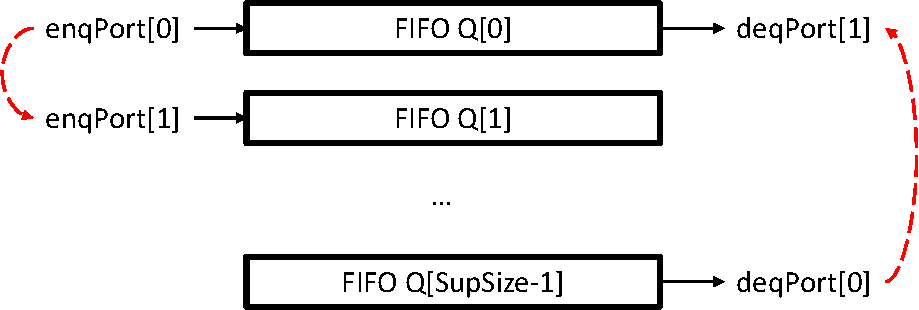
\includegraphics[width=0.6\columnwidth]{fig/rob_rotate_fifos_crop.pdf}
    \caption{Organizing ROB entries a set of FIFOs}\label{fig:rob-rotate-fifos}
\end{figure}

With the above implementation, each dequeue/enqueue only access a single FIFO, which has $N$/\code{SupSize} entries.
We also need to rotate the enqueue or dequeue data to match the correct FIFOs, and this rotation will cost $O($\code{SupSize}$)$ units of area.
Thus, the total area cost is $N +O($\code{SupSize}$)$ units of area.

Methods \code{setExecuted\_XXX}, \code{setLSQAtCommitNotified}, \code{getOrig} and \code{correctSpeculation} access the EHRs for ROB entries directly.
However, methods \code{deqPort}, \code{enqPort}, and \code{incorrectSpeculation} do not access EHRs directly.
These three methods simply record their arguments in wires, and the real actions are taken in three canonicalize rules, i.e., \code{canon\_deq}, \code{canon\_enq}, and \code{canon\_wrongSpec}, respectively.
Using canonicalize rules makes it easy to handle superscalar enqueues and dequeues.
The canonicalize rules enforce the ordering semantics of the conflict matrix and we artificially impose orderings between these methods (e.g., by reading and writing dummy registers).
The following orderings need to be created artificially:
\begin{itemize}
    \item \code{deqPort} $<$ \code{enqPort}
    \item \code{setExecuted\_XXX} $<$ \code{enqPort}
    \item \code{setLSQAtCommitNotified} $<$ \code{enqPort}
    \item \code{incorrectSpeculation} C \code{enqPort}
    \item \code{deqPort} $<$ \code{incorrectSpeculation}
\end{itemize}

\noindent\textbf{Conflict Matrix:}
The conflict matrix for the methods and rules that access EHRs directly is the following:
\begin{itemize}
    \item \code{canon\_deq} $<$ \code{setExecuted\_XXX} $<$ \code{canon\_enq} $<$ \code{correctSpeculation}
    \item \code{canon\_deq} $<$ \code{setLSQAtCommitNotified} $<$ \code{canon\_enq}
    \item \code{canon\_enq} mutually exclusive with \code{canon\_wrongSpec}
    \item \code{canon\_deq} $<$ \code{canon\_wrongSpec} $<$ \code{correctSpeculation}
\end{itemize}
These methods and rules will access EHRs using the ports according to this conflict matrix

Since other methods are conflict free with each other, they may either directly access the EHRs with port 0 or access indirectly using wires.

We also made one slight optimization on the guard signal of \code{enqPort}.
That is, the evaluation of the enqueue guard ignores the effects of dequeues.
This cut off the combinational path from dequeue to enqueue.

\subsubsection{Source Code}
See the following:
\begin{itemize}
    \item module \code{mkReorderBufferSynth} in file \code{//procs/RV64G\_OOO/ReorderBufferSynth.bsv}, and
    \item module \code{mkSupReorderBuffer} in file \code{//procs/lib/ReorderBuffer.bsv}.
\end{itemize}

\subsubsection{Future Improvement}
Below are the possible future improvements:
\begin{itemize}
    \item Order methods \code{getOrigPredPC}, \code{getOrigPC} and \code{getEnqTime} before \code{enqPort} as explained above.
    
    \item See if it is possible for \code{enqPort}, \code{deqPort} and \code{incorrectSpeculation} methods to directly access EHRs.
    This can reduce the amount of wires.
    How much is the cost of doing so?
    
    \item Explore alternative organizations of ROB entries. Can we get some information about commercial designs?
\end{itemize}